\documentclass[border=4pt]{standalone}
\usepackage{tikz}
\usetikzlibrary{calc,shapes.geometric}

\begin{document}
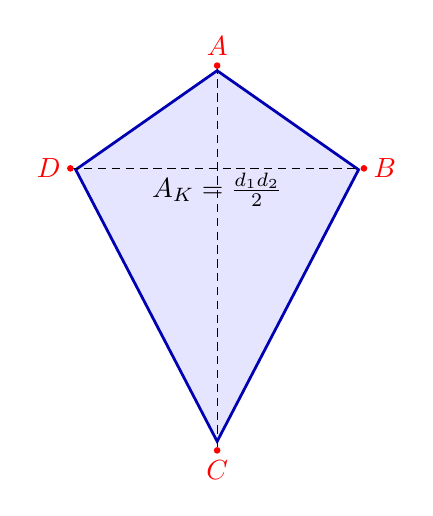
\begin{tikzpicture}
  \node[kite,kite upper vertex angle=110,kite lower vertex angle=55,
    minimum width=36mm,minimum height=46mm,draw=blue!70!black,
    fill=blue!10,line width=1pt,outer sep=1.5pt] (K) at (0,0) {};
  \draw[densely dashed] (K.upper vertex) -- (K.lower vertex);
  \draw[densely dashed] (K.left vertex) -- (K.right vertex);
  \fill[red] (K.upper vertex) circle (1.2pt) node[above] {$A$};
  \fill[red] (K.right vertex) circle (1.2pt) node[right] {$B$};
  \fill[red] (K.lower vertex) circle (1.2pt) node[below] {$C$};
  \fill[red] (K.left vertex) circle (1.2pt) node[left] {$D$};
  \node at ($(K.center)+(0,-2mm)$) {$A_K=\frac{d_1d_2}{2}$};
\end{tikzpicture}
\end{document}
